\documentclass[tikz, border=10pt]{standalone}
\usepackage{circuitikz}
\usepackage{tikz-dimline}
\usetikzlibrary{patterns, positioning, calc}
\usepackage{tikz-cd}

% Plot caching
\usetikzlibrary{external}
\tikzexternalize[]

% Fonts
\usepackage{fontspec}

\setmainfont{Trebuchet MS}[
    Path = fonts/,
    UprightFont    = trebuc.ttf,
    BoldFont       = trebucbd.ttf,
    ItalicFont     = trebuci.ttf,
    BoldItalicFont = trebucbi.ttf
]

\begin{document}

\tikzcdset{background color=none}
% \begin{tikzpicture}[scale=1.0, font=\sffamily]



%     % --- 1. Configuration ---
%     \def\gateW{3}       % Gate Width
%     \def\gateH{8}       % Gate Height
%     \def\overlap{0.6}   % Overlap Width
%     \def\wireY{3.2}     % Height of the capacitor wire
%     \definecolor{overlapBlue}{RGB}{173, 216, 230}

%     % --- 2. Diffusion Regions ---
%     \draw[pattern=north east lines, pattern color=black, line width=1pt] 
%         (-5, -2) rectangle (-1.5, 2); % Source
%     \draw[pattern=north east lines, pattern color=black, line width=1pt] 
%         (1.5, -2) rectangle (5, 2);   % Drain

%     % --- 3. Gate ---
%     \draw[fill=white, line width=1.5pt] (-1.5, -4) rectangle (1.5, 4);

%     % --- 4. Overlap Regions ---
%     \draw[fill=overlapBlue, line width=1pt] (-1.5, -2) rectangle (-1.5 + \overlap, 2);
%     \draw[fill=overlapBlue, line width=1pt] (1.5 - \overlap, -2) rectangle (1.5, 2);

%     % --- 5. Labels ---
%     \node[below] at (-3.25, -2.2) {\large \textbf{Source}};
%     \node[below] at (3.25, -2.2) {\large \textbf{Drain}};
%     \node[below] at (0, -4.2) {\large \textbf{Gate}};

%     % --- 6. Capacitors (Circuitikz) ---
%     % Define dots
%     \coordinate (S_dot) at (-3.5, 0);
%     \coordinate (D_dot) at (3.5, 0);
%     \coordinate (G_dot_S) at (-0.5, 0);
%     \coordinate (G_dot_D) at (0.5, 0);
    
%     \filldraw (S_dot) circle (4pt) (D_dot) circle (4pt) 
%               (G_dot_S) circle (4pt) (G_dot_D) circle (4pt);

%     % Global style for thicker capacitor plates
%     \ctikzset{bipoles/thickness=1.5}

%     % C_GS: Path goes Right -> Label 'l' is on top (Left of path)
%     \draw[line width=1.5pt] (S_dot) -- (-3.5, \wireY) 
%         to[C, l=$\mathbf{C_{GS}}$, thick] (-0.5, \wireY) 
%         -- (G_dot_S);

%     % C_GD: Path goes Left -> Label 'l_' (underscore) puts it on top (Right of path)
%     \draw[line width=1.5pt] (D_dot) -- (3.5, \wireY) 
%         to[C, l_=$\mathbf{C_{GD}}$, thick] (0.5, \wireY) 
%         -- (G_dot_D);

%     % \draw[Cote arrow,-] 1 -- 2;

% \end{tikzpicture}

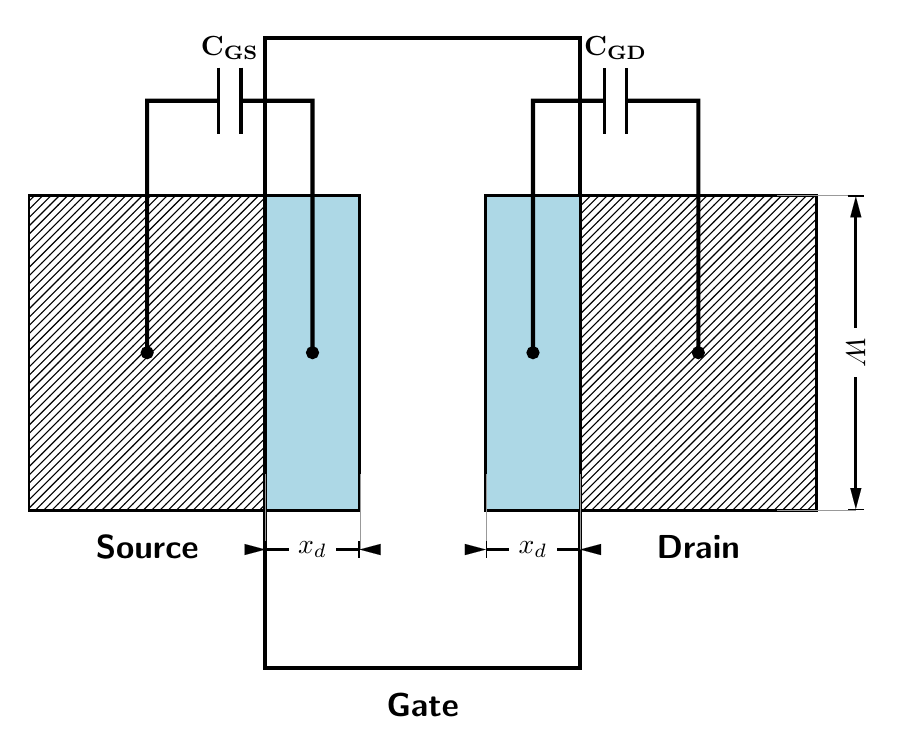
\begin{tikzpicture}[scale=1.0, font=\sffamily]

    % --- 1. Configuration ---
    \def\gateW{4}       % Gate Width
    \def\gateH{8}       % Gate Height
    \def\diffW{3}       % Diffusion Width
    \def\diffH{4}       % Diffusion Height
    \def\overlap{1.2}   % Overlap Width
    \def\wireY{3.2}     % Height of the capacitor wire
    \definecolor{overlapBlue}{RGB}{173, 216, 230}

    \def\sourceLeft{-5}
    \def\sourceBottom{-2}
    \def\drainBottom{\sourceBottom}
    \def\gateLeft{\sourceLeft+\diffW}
    \def\drainLeft{\gateLeft+\gateW}
    \def\gateBottom{-\gateH/2}

    % --- 2. Diffusion Regions ---
    \draw[pattern=north east lines, pattern color=black, line width=1pt] 
        (\sourceLeft, \sourceBottom) rectangle +(\diffW,\diffH); % Source
    \draw[pattern=north east lines, pattern color=black, line width=1pt] 
        (\drainLeft, \drainBottom) rectangle +(\diffW, \diffH);   % Drain

    % --- 3. Gate ---
    \draw[fill=white, line width=1.5pt] (\gateLeft, \gateBottom) rectangle +(\gateW,\gateH);

    % --- 4. Overlap Regions ---
    % Source Overlap
    \draw[fill=overlapBlue, line width=1pt] (\gateLeft, \sourceBottom) rectangle +(\overlap, \diffH);
    % Drain Overlap
    \draw[fill=overlapBlue, line width=1pt] (\drainLeft, \drainBottom) rectangle +(-\overlap, \diffH);

    \coordinate (S_dot) at (\sourceLeft+\diffW/2, 0);
    \coordinate (D_dot) at (\drainLeft+\diffW/2, 0);
    \coordinate (G_dot_S) at (\gateLeft+\overlap/2, 0);
    \coordinate (G_dot_D) at (\drainLeft-\overlap/2, 0);

    % --- 5. Text Labels (Regions) ---
    \node[below] at ($(S_dot)-(0,\diffH/2+0.2)$) {\large \textbf{Source}};
    \node[below] at ($(D_dot)-(0,\diffH/2+0.2)$) {\large \textbf{Drain}};
    \node[below] at (\gateLeft+\gateW/2,-\gateH/2-0.2) {\large \textbf{Gate}};

    % --- 6. Capacitors (Circuitikz) ---
    
    % \filldraw (S_dot) circle (2pt) (D_dot) circle (2pt) 
              % (G_dot_S) circle (2pt) (G_dot_D) circle (2pt);

    \ctikzset{bipoles/thickness=1.5}

    % C_GS
    \draw[line width=1.5pt] (S_dot) node[circ]{} -- ++(0, \wireY) to[C, l=$\mathbf{C_{GS}}$, thick] (G_dot_S |- \tikztostart) to (G_dot_S) node[circ]{};

    % C_GD
    \draw[line width=1.5pt] (D_dot) node[circ]{} -- ++(0, \wireY) 
        to[C, l_=$\mathbf{C_{GD}}$, thick] (G_dot_D |- \tikztostart) 
        -- (G_dot_D) node[circ]{};

    \coordinate (sOverlapTL) at (\gateLeft,-\diffH/2 - 0.5);
    \coordinate (sOverlapTR) at (\gateLeft+\overlap,-\diffH/2 - 0.5);
    \coordinate (dOverlapTR) at (\drainLeft,-\diffH/2 - 0.5);
    \coordinate (dOverlapTL) at (\drainLeft-\overlap,-\diffH/2 - 0.5);
    
    % \coordinate (sOverlapTL) at (\gateLeft,\diffH/2);
    % \coordinate (sOverlapTR) at (\gateLeft+\overlap,\diffH/2);
    % \coordinate (dOverlapTR) at (\drainLeft,\diffH/2);
    % \coordinate (dOverlapTL) at (\drainLeft-\overlap,\diffH/2);

    \coordinate (wEnd) at (\drainLeft+\diffW+0.5,\drainBottom);
    \coordinate (wStart) at (\drainLeft+\diffW+0.5,\drainBottom+\diffH);

    \dimline[line style = {line width=1}, label style={fill=white}]{(wStart)}{(wEnd)}{$W$};

    \dimline[
        line style = {
            line width=1, 
            arrows=dimline reverse-dimline reverse
        }, 
        extension start length=-0.8, 
        extension end length=-0.8, 
        label style={
            fill=white
        }
    ]{(sOverlapTL)}{(sOverlapTR)}{$x_d$};

    \dimline[
        line style = {
            line width=1, 
            arrows=dimline reverse-dimline reverse
        }, 
        extension start length=-0.8, 
        extension end length=-0.8, 
        label style={
            fill=white
        }
    ]{(dOverlapTL)}{(dOverlapTR)}{$x_d$};

\end{tikzpicture}

\end{document}